%-----------------------------------------------
% Template para criação de resumos de projectos/dissertação
% jlopes AT fe.up.pt,   Fri Jul  3 11:08:59 2009
%-----------------------------------------------

\documentclass[9pt,a4paper]{extarticle}

%% English version: comment first, uncomment second
\usepackage[portuguese]{babel}  % Portuguese
%\usepackage[english]{babel}     % English
\usepackage{graphicx}           % images .png or .pdf w/ pdflatex OR .eps w/ latex
\usepackage{times}              % use Times type-1 fonts
\usepackage[utf8]{inputenc}     % 8 bits using UTF-8
\usepackage{url}                % URLs
\usepackage{multicol}           % twocolumn, etc
\usepackage{float}              % improve figures & tables floating
\usepackage[tableposition=top]{caption} % captions
%% English version: comment first (maybe)
\usepackage{indentfirst}        % portuguese standard for paragraphs
%\usepackage{parskip}
\usepackage{array}
\newcolumntype{M}{ >{\centering\arraybackslash} m{0.7cm} }
\newcolumntype{C}{ >{\centering\arraybackslash} m{2cm} }
%% page layout
\usepackage[a4paper,margin=30mm,noheadfoot]{geometry}

%% space between columns
\columnsep 12mm

%% headers & footers
\pagestyle{empty}

%% figure & table caption
\captionsetup{figurename=Fig.,tablename=Tab.,labelsep=endash,font=bf,skip=.5\baselineskip}

%% heading
\makeatletter
\renewcommand*{\@seccntformat}[1]{%
  \csname the#1\endcsname.\quad
}
\makeatother

%% avoid widows and orphans
\clubpenalty=300
\widowpenalty=300

\begin{document}

\title{\vspace*{-8mm}\textbf{\textsc{Online Advertising: Forecasting and Synthesising Web Activity Based On Historical Data}}}
\author{\emph{Pedro Manuel Santos Borges}\\[2mm]
\small{Dissertação desenvolvida sob a supervisão do Prof. João Moreira, co-supervisão do Prof. Hugo Ferreira}\\
\small{e supervisão da empresa do Eng. João Azevedo}\\
\small{na \emph{ShiftForward, Lda}}}
\date{}
\maketitle
%no page number 
\thispagestyle{empty}

\vspace*{-4mm}\noindent\rule{\textwidth}{0.4pt}\vspace*{4mm}

\begin{multicols}{2}

\section{Enquadramento e Contexto} \label{sec:context}


O marketing online é uma indústria multibilionária em grande
crescimento\cite{PricewaterhouseCoopers2013} na qual é expectável a
continuidade desse mesmo crescimento rápido\cite{PricewaterhouseCoopers2013a}.

Esta indústria tenta constantemente tornar-se mais eficiente, maximizando o
lucro de ativos que já possui. Os utilizadores da Internet são os principais
ativos dessa indústria, que ganha dinheiro explorando o seu comportamento e
características, a fim de os atingir com a campanha perfeita. Cada campanha tem
seus próprios parâmetros e regras, que limitam o universo de utilizadores-alvo.

O foco da indústria de marketing on-line são os utilizadores da internet e por
isso, regista todos os rastos que estes deixam na internet. As acções futuras
dos utilizadores da Internet permitem a medição do comportamento de uma
campanha futura e, tendo acesso a esses dados, é possível tornar o inventário
mais rentável. Portanto, o uso destes dados permite à indústria de publicidade
online ajustar suas campanhas futuras de forma a melhor atingir o seu publico
alvo. As campanhas são compostas por uma série de anúncios que partilham a mesma
idéia principal que se quer transmitir. Para ser possível simular as campanhas num
simulador estás são definidas
como um conjunto de \emph{queries} sobre um \emph{dataset de
utilizadores}. A utilização de uma simulação permite obter resultados rápidos,
testar campanhas simultâneas e testar vários cenários possíveis. A utilização
de uma simulação é a principal razão que justifica a necessidade de gerar dados
que representem os pedidos efectuados por cada utilizador.

As plataformas mais comuns que beneficiarão destes resultados são
\emph{Custom-Built Ad Servers and Exchanges}, \emph{Sell-Side Platforms} (SSPs)
and \emph{Demand-Side Platforms}(DSPs).

\section{Projecto} \label{sec:proj}

O objectivo deste projecto é prever a disponibilidade de utilizadores no futuro
para podermos simular campanhas publicitarias sobre eles.

Sendo que à partida não sabemos que características vão ter as campanhas,
precisamos de prever todas as caracteristicas dos utilizadores de forma a
conseguir determinar os volumes para cada campanha, através de \emph{queries}
sobre os dados gerados. 

O principal objectivo deste projecto é gerar um conjunto de dados que possa ser
usado num simulador de campanhas, por isso temos que prever os valores com o
máximo detalhe.

Este simulador precisa de ter disponível todos os detalhes que compões uma
entrada no conjunto de dados (\emph{impression}), a dim de conseguir
identificar que utilizador vai ser atingido por cada campanha. O resultado
seria expresso pelo número de impressões por campanha e pelo numero de
utilizadores únicos atingidos, ao longo do tempo.

Esta abordagem tem que ser capaz de utilizar apenas a data de uma impressão e
ID do utilizadores, com todas as outras variáveis opcionais. Essa restrição é
imposta pelas múltiplas origens que o conjunto de dados pode ter, uma vez que
cada uma destas fontes pode armazenar detalhes diferentes e diferentes tipos de
parâmetros sobre cada impressão, deste modo não podemos contar com a
disponibilidade de algum parâmetro além destes dois.

\section{Motivação e Objectivos} \label{sec:goals}

Nos últimos anos, o marketing online tem vindo a tornar-se um mercado mais
complexo. De tal forma que hoje as campanhas tem um alvo muito bem definido,
por regras e limitações. Isto representa um grande problema para os modelos de
previsão mais simples. Estes normalmente não prevêem todos os parâmetros de um
pedido de publicidade, diminuindo assim a informação disponível para cálculos
de performance de uma campanha.

Algumas campanhas hoje em dia são muito especificas, mesmo em termos temporais,
como por exemplo, os utilizadores que visitaram um site de e-commerce nas
últimas 24 horas. Isto traz causalidade na equação, criando um novo paradigma,
que faz os métodos mais tradicionais de previsão ineficazes. Para resolver este
problema e ser capaz de obter respostas rápidas a consultas complexas de
campanhas simultâneas, simulando os algoritmos executados por servidores de
anúncios do cliente e, finalmente, paralelizar o cálculo dos resultados para o
consultas, os pedidos futuros tem que estar disponíveis. 

O objetivo deste trabalho é desenvolver uma biblioteca capaz de gerar pedidos
futuros de anúncios usando dados do passado da mesma rede. Esta biblioteca tem
como um de seus principais objetivos a previsão de todos os parâmetros que
caracterizam um pedido de anúncio. Para que o conjunto de pedidos gerados possa
ser usado para consulta sobre qualquer parâmetro, ou seja, o conjunto de dados
gerados (registo de pedidos) deve ter disponível os mesmo parâmetros que o
original.

\section{Abordagem}

\begin{figure}[H]
\centering
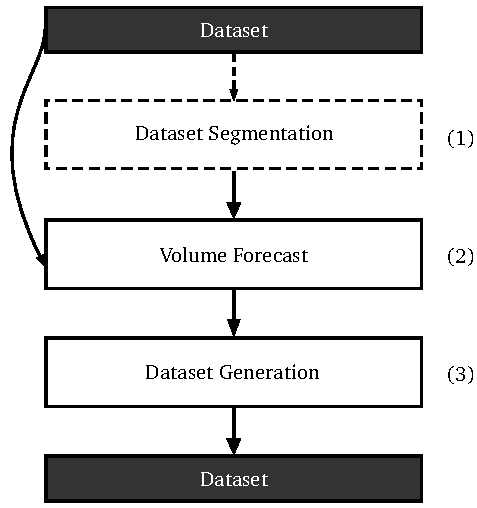
\includegraphics[width=0.25\textwidth]{high_level} \caption{Arquitectura de alto
nivel da abordagem} \label{fig:highlevel_arch} \end{figure}

Como representado na Figura~\ref{fig:highlevel_arch} mostra, o objectivo da
abordagem proposta é gerar os dados futuros dos pedidos numa rede relacionada
com a publicidade online, usando apenas registos passados.
Esta previsão deve manter as tendências do passado e manter coerência dos dados.

A abordagem pode ser dividida em três fases principais:
\begin{enumerate}
\item \emph{Segmentação}, o principal objectivo desta fase é dividir os dados
  em subconjuntos, mais pequenos e mais previsíveis, a fim de melhorar os
  resultados das fases seguintes, principalmente quando há muitos dados
  disponíveis.

\item A segunda fase compreende a \emph{revisão dos volumes}, de valores que
  caracterizam o tráfego da rede, usando métodos de previsão de series
  temporais(usando por exemplo \emph{ARIMA}).

\item A terceira fase do processo, utiliza os valores gerados pelas duas fases
  anteriores e combinando-os com o conjunto de dados do passado,
  \emph{gerar um conjunto de dados} que representa um possível futuro do trafego da rede. 
\end{enumerate}

\section{Resultados}

\begin{table}[H]
\centering
\footnotesize
\begin{tabular}{m{2cm}|CMM}
  &  $\sigma$ (Dados reais) & RMSE & MASE   \\ \hline
 Sem segmentação & 2224.74 & 1237.99 & 0.1958 \\ \hline
  \emph{baseline} (100 segmentos) & 2224.74 & 1352.42 & 0.2174 \\ \hline
  segmentação por parametro (\emph{browser}) & 2224.74 & 1226.60 & 0.1884 \\ \hline
  segmentação por \emph{datastream clustering} (\emph{threshold} 20) & 2224.74 & 1786.43 & 0.2927 \\ \hline
\end{tabular}

\caption[]{Previsão para o volume de impressões de um conjunto de dados real}
\label{tab:noquery}
\end{table}

\begin{table}[H]
\centering
\footnotesize
\begin{tabular}{m{2cm}|CMM}
  &  $\sigma$ (Dados reais) & RMSE & MASE   \\ \hline
 Sem segmentação & 6.70 & 9.24 & 1.2511 \\ \hline
 \emph{baseline} (100 segmentos) & 6.70 & 6.88 & 0.7896 \\ \hline
 segmentação por parametro (\emph{browser}) & 6.70 & 10.75 & 1.3883 \\ \hline
 segmentação por \emph{datastream clustering} (\emph{threshold} 20) & 6.70 & 15.93 & 2.5960 \\ \hline
\end{tabular}

\caption[]{Previsão para o volume de impressões de um conjunto de dados real, pesquisa por
''Portugal''}
\label{tab:query}
\end{table}

Em praticamente todos os casos de teste obtiveram melhores resultados quando a
fase de segmentação foi realizada(alguns exemplos na tabela~ref{tab:noquery}
and ~\ref{tab:query}). Os resultados calculados foram apenas num número pequeno
de pesquisas, podendo ter um resultado diferente quando usados no ambiente de
simulador.

\section{Cumprimento dos Objectivos}

Propomos o uso das três fases. A primeira fase permite melhores previsões para
determinadas características, a segunda permite prever os volumes futuros dos
valores que caracterizam o conjunto de dados e, finalmente, a terceira fase
preenche o conjunto futuro usando os volumes previstos e seguindo as tendências
e dados fornecidas pelo conjunto de dados do passado. Os nossos resultados
demostram um melhoria moderada dos resultados quando é feita segmentação.

\section{Trabalho futuro}

Diferentes abordagens em cada fase poderiam ser exploradas de forma a obter
melhores resultados. Na fase de segmentação outros algoritmos de segmentação
poderiam ser utilizados, por exemplo segmentação recursiva por parâmetro.
Acredito que esta abordagem teria bons resultados quando muitos dados
estivessem disponíveis.
Na previsão de volumes outras techiniques e algoritmos poderam ser testados
como por exemplo \emph{MLP}, \emph{multilayer perceptron}.
Na fase de gerar o conjunto de dados, conhecimento adicional sobre como cada
parametro é construido poderia ser usado em conjunto com novas metricas
(percentagem de novas cidades, por exemplo).

%%English version: comment first, uncomment second
\bibliographystyle{unsrt-pt}  % numeric, unsorted refs
%\bibliographystyle{unsrt}  % numeric, unsorted refs
\bibliography{refs}

\end{multicols}

\end{document}
